\documentclass[Slovak, a4paper, 12pt]{article}

\usepackage[slovak]{babel}
\usepackage[text={17cm, 24cm}, top=3cm, left = 2cm]{geometry}
\usepackage[T1]{fontenc}
\usepackage[utf8]{inputenc}
\usepackage{times}
\usepackage{graphics}
\usepackage{wrapfig}

\begin{document}
	\begin{titlepage}
		
		\begin{center}
			\textsc{{\LARGE Vysoké učení technické v Brně \\[0.5em]}  {\LARGE Fakulta informačních technologií}} \\
			\vspace{\stretch{0.382}}
			{\Large Formálne jazyky a prekladače  -- Projekt \\[0.6em]}
			{\huge Prekladač pre jazyk ZIG} \\[0.6em]
			{\large Tým xluptas00 varianta TRP-izp}
			\vspace{\stretch{0.618}}
			
		\end{center}
		\begin{flushright}
			{ \textbf{Bodové rozdelenie:} 25/25/25/25\% \hfill \textbf{Vedúci: }Samuel Lupták (xluptas00)} \\
			{ \textbf{Implementované rozšírenia:} žiadne\hfill  Petr Nemec (xnemecp00)} \\
			{ \hfill  Lukáš Houzar (xhouzal00)} \\
			{\today \hfill Mário Klopan (xklopam00)}
		\end{flushright}
		
	\end{titlepage}
	
	\section{Návrh}
	\noindent Prekladač sa skladá z 3~hlavných častí a 4~pomocných dátových štruktúr.\\
	\textbf{Hlavné časti} prekladaču (a ich podčasti):
	\begin{itemize}
		\item Lexikálny analyzátor \footnote[1]{Ďalej len \textit{skener}}
		\item Dvojprechodový syntaktický a sématický analyzátor \footnote[2]{Ďalej len \textit{parser}}
		\begin{itemize} 
			\item Analýza kódu pomocou rekurzívneho zostupu
			\item Analýza výrazov pomocou precedenčnej analýzi 
		\end{itemize}
		\item Generátor výsledného kódu
	\end{itemize}
	
	\noindent\textbf{Pomocné štruktúry} použité v prekladači:
		\begin{itemize}
		\item  Tabulka s rozptýlenými položkami s implicitným zreťazením položiek \footnote[3]{Ďalej len \textit{hašovacia tabulka}}
		\item Abstraktný syntaktický strom \footnote[4]{Ďalej len \textit{ASS}}
		\item Zásobník
		\item Fronta
	\end{itemize}
	
	\noindent \textbf{Využitie} jednotlivých štruktúr je nasledovné:\\
	\par\textit{Hašovacia tabulka: } Bola použítá pre implementáciu tabulky symbolov. Podmienka pre implicitné zreťazenie nám 
	robila mierny problém, pretože teoreticky nekonečný počet identifikátorov sa nemestí do konečne velkej tabulky \\
	\par\textit{ASS: } Slúži na komunikáciu medzi parserom a generátorom kódu\\
	\par\textit{Zásobník: } Je využitý precedenčnou analýzou, ktorá ho používa na spracovanie výrazov\\
	\par\textit{Fronta: } Má význam pri dvojprechodovej analýze ako uložisko tokenov. Pre dvojprechodovú analýzu sme sa rozhodli po
	zistení, že definicia funkcie nemusí lexikálne predchádzať jej volaniu.
	
	\newpage
	\section{Popis komunikácie}
	\subsection{Diagram}
	
	\begin{figure}[ht]
		\begin{center}
			\scalebox{0.5}{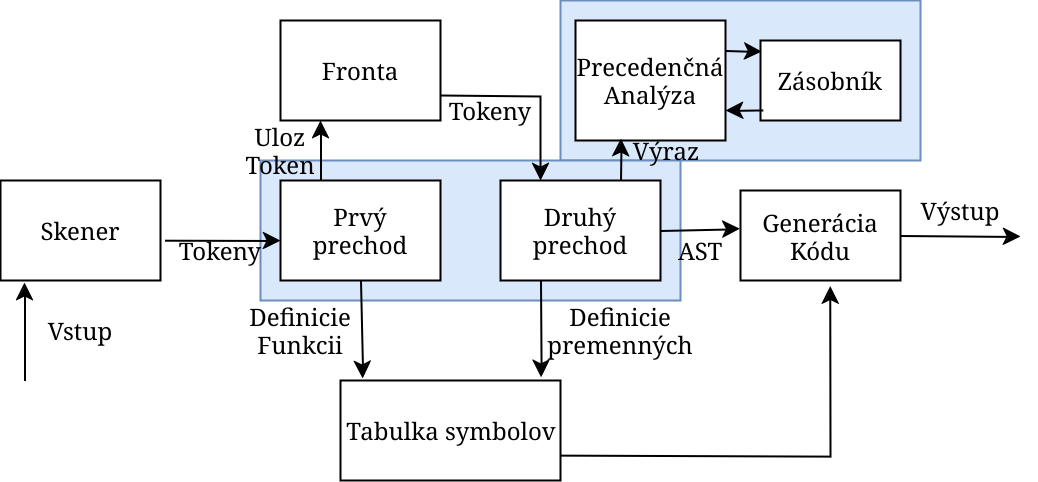
\includegraphics{Untitled Diagram.png}}
			\caption{Diagram komunikácie}
		\end{center}
	\end{figure}
	\subsection{Stručný popis}
	Bolo by vhodné začať tým, že parser (modrá časť diagramu) inicializuje všetky operácie v prekladači.  
	Preklad začína vložením programu v jazyku zig na
	 vstup. Skener (Na zavolanie) postupne fragmentuje vstup na jednotlivé lexémi a posiela ich vo forme tokenov do parseru.  Ako bolo už spomenuté, tak parser je dvojprechodový. Tokeny idú najprv cez prvý prechod, ktorý kontroluje syntax a sematiku iba pre hlavičky funkcií, ktoré následne ukladá do tabulky symbolov, aby informácie o nich boli dostupné v druhom prechode. Prvý prechod ukladá všetky prečítané tokeny do fronty. Z fronty si tokeny po jednom berie druhý prechod, ktorý kontroluje syntax a sématiku pre ostatok kódu. V prípade že v kóde sa nachádza výraz, zavolá sa precedenčná analýza ktorá tento výraz s pomocov zásobníku spracuje. Druhý prechod zároveň pridáva definované premenné do tabulky symbolov  (Samotnú tabulku symbolov však aj využíva, napr. pre kontrolu redefinície).  Počas druhého prechodu sa zároveň vytvára ASS ktorý po úspešnom dokončení analýzi slúži ako výstup a zároveň vstup do generátoru kódu. Generátor kódu s pomocou tabulky symbolou generuje cieľový kód.
	 	
	\newpage
	\section{Implementácia}
	\textbf{Skener: }\textit{lexer.*, token.h} (xhouzal00, xnemecp00)\\ 
	\textbf{Parser: }\textit{syntax.*, queue\_fill.*, precedence.*} (xluptas00, xklopam00)\\
	\textbf{Generátor kódu: }\textit{code\_gen.*} (xhouzal00, xnemecp00)\\
	\textbf{Hašovacia tabulka: }\textit{symtable.*} (xluptas00)\\
	\textbf{ASS: }\textit{tree.*} (xklopam00)\\
	\textbf{Zásobník: }\textit{stack.*} (xklopam00)\\
	\textbf{Fronta: }\textit{queue.*} (xluptas00)\\
	\textbf{Ostatné časti: }\textit{error.*} (xluptas00)\\
	\par Implementácia dátových štruktúr sa nachádza v jednotlitvých súboroch pomenovaných podla danej štruktúry.
	\par Implementácia častí samotného prekladača spočíva v súboroch skeneru, parseru, generátoru a súboru \textit{error.*}, ktorý 
	implementuje základné pracovanie s chybami. Prvý prechod je implementovaný v súboroch \textit{queue\_fill.*} a druhý prechod je
	implementovaný v súboroch \textit{syntax.*}. \textit{syntax.c} zároveň obsahuje funkciu Main. Prílohy A, B, C, D ukazujú využitú teóriu, ktorá slúžila ako podklad pre jednotlivé časti prekladaču.
	\subsection{Strom}
	\begin{wrapfigure}{l}{0.4\textwidth}
		\scalebox{0.25}{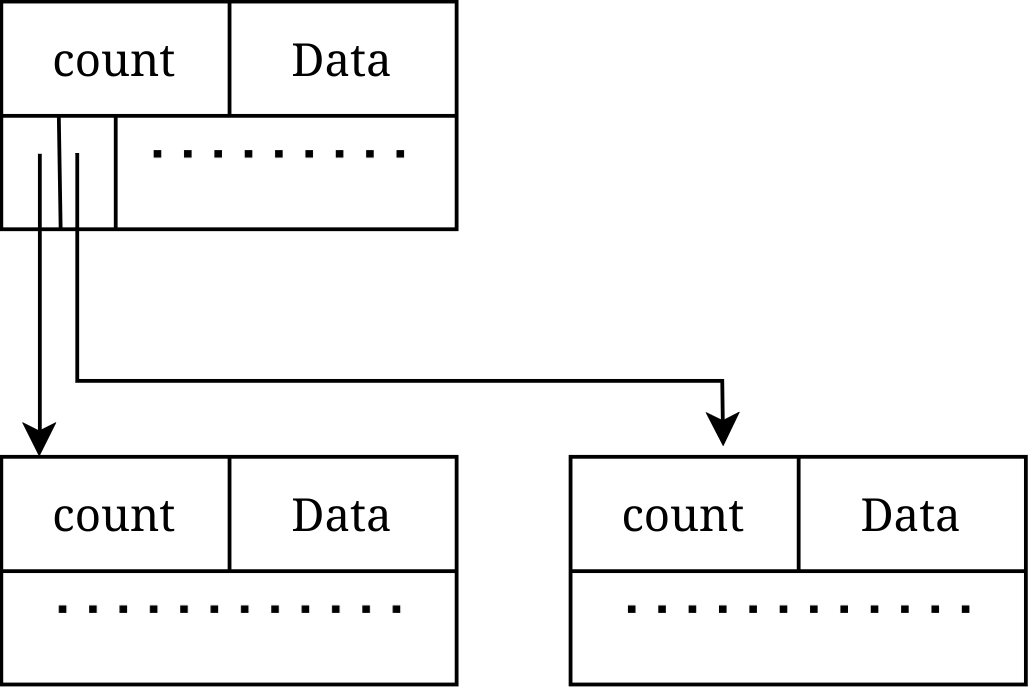
\includegraphics{Untitled Diagram(1).png}}
		\caption{Štruktúra stromu}
	\end{wrapfigure}
	Pre kompletnosť sme sa rozhodli vizualizovať ASS, ktorý sme navrhli pre tento prekladač.
	Ako je vidno na diagrame, tak každý uzol obsahuje 3 hlavné časti a to sú: \textit{count, data, children}. Kde \textit{count}
	určuje počet detí ktoré daný uzol má. Hlavná časť, \textit{data}, v sebe uchováva data potrebné na správne generovanie kódu
	(viac viď. tree.*). Posledná časť \textit{children} je pole ukazovaťelov na deti.  V texte ďalej ukážeme ako sa "kódujú" jednotlivé časti kódu do tohto stromu.
	\\\\
	\textbf{Typy uzlov} sú špecifikované v \textit{tree.h:15}. Strom má presne 1 koreň typu \textbf{ROOT\_NODE}  a má presne tolko detí, kolko je funkcií vo
	vstupnom programe. Tieto uzly sú typu \textbf{TOP\_FUNCTION\_NODE} a sú v nich uložené základné informácie o funkciách potrebné pre generáciu kódu.
	Z jednotlivých uzlov funkcií vychádzajú uzly špecifikujúce jednotlivé časti kódu. Tieto časti kódu sa delia na: \textit{priradenie, definiciu premennej, návrat, vetvenie, cyklus, volanie funkcie}. \\[0.6em]
	\textit{Priradenie} začína uzlom \textbf{ASSIGN\_NODE}, jeho prvé dieťa určuje do akej premennej sa priraďuje a jeho druhé dieťa určuje čo sa priraďuje (funkcia alebo výraz).\\[0.6em]
	\textit{Definicia premennej} má ten istý tvar ako \textit{priradenie} až na to že vrchný uzol má typ \textbf{DEFINITION\_NODE}\\[0.6em]
	\textit{Návrat} začina uzlom typu \textbf{RETURN\_NODE} . Jeho jedniným dieťaťom je strom výrazu, v prípade funkcie nevracajúcej hodnotu nemá deti žiadne.\\[0.6em]
	\textit{Vetvenie} a \textit{cyklus} začínajú uzlom typu \textbf{WHILE\_NODE} alebo \textbf{IF\_NODE}. Na prvom mieste sa nachádza podmineka.  Následuje postupnosť častí kódu. Pokiaľ sa jedná o podmineku, začiatok druhej vetvy označuje dieťa typu \textbf{ELSE\_NODE} následovaná postupnosťou častí kódu.\\[0.6em]
	\textit{Volanie funkcie} začína uzlom \textbf{FUNCTION\_NODE} a jeho deti sú postupnosť argumentov. Podobne fungujú aj vstavané funkcie s miernou zmenou 
	typu hlavného uzlu\\[0.6em]
	\noindent Zauimavým doplnkom stromu je inklúzia spätného odkazu na otca v každdom uzle. Toto umožňuje celkom elegantné zarovanie a vynorovanie v 
	rekurzívnom zostupe. Pokiaľ je napríklad volaná funkcia, program sa zanorý do uzlu \textbf{FUNCTION\_NODE} a zaplní ho uzlami argumentov. po jeho spracovaní sa pomocov spätného odkazu program vynorí z tohto uzlu a je pripravený spracovať ďalšie riadky kódu.\\[0.6em]
	\noindent \textit{Generácia kódu} následne generuje kód jednoduchým prechádzaním tohoto stromu.
	
	\subsection{Tabulka symbolov}
		\begin{wrapfigure}{l}{0.35\textwidth}
			\scalebox{0.2}{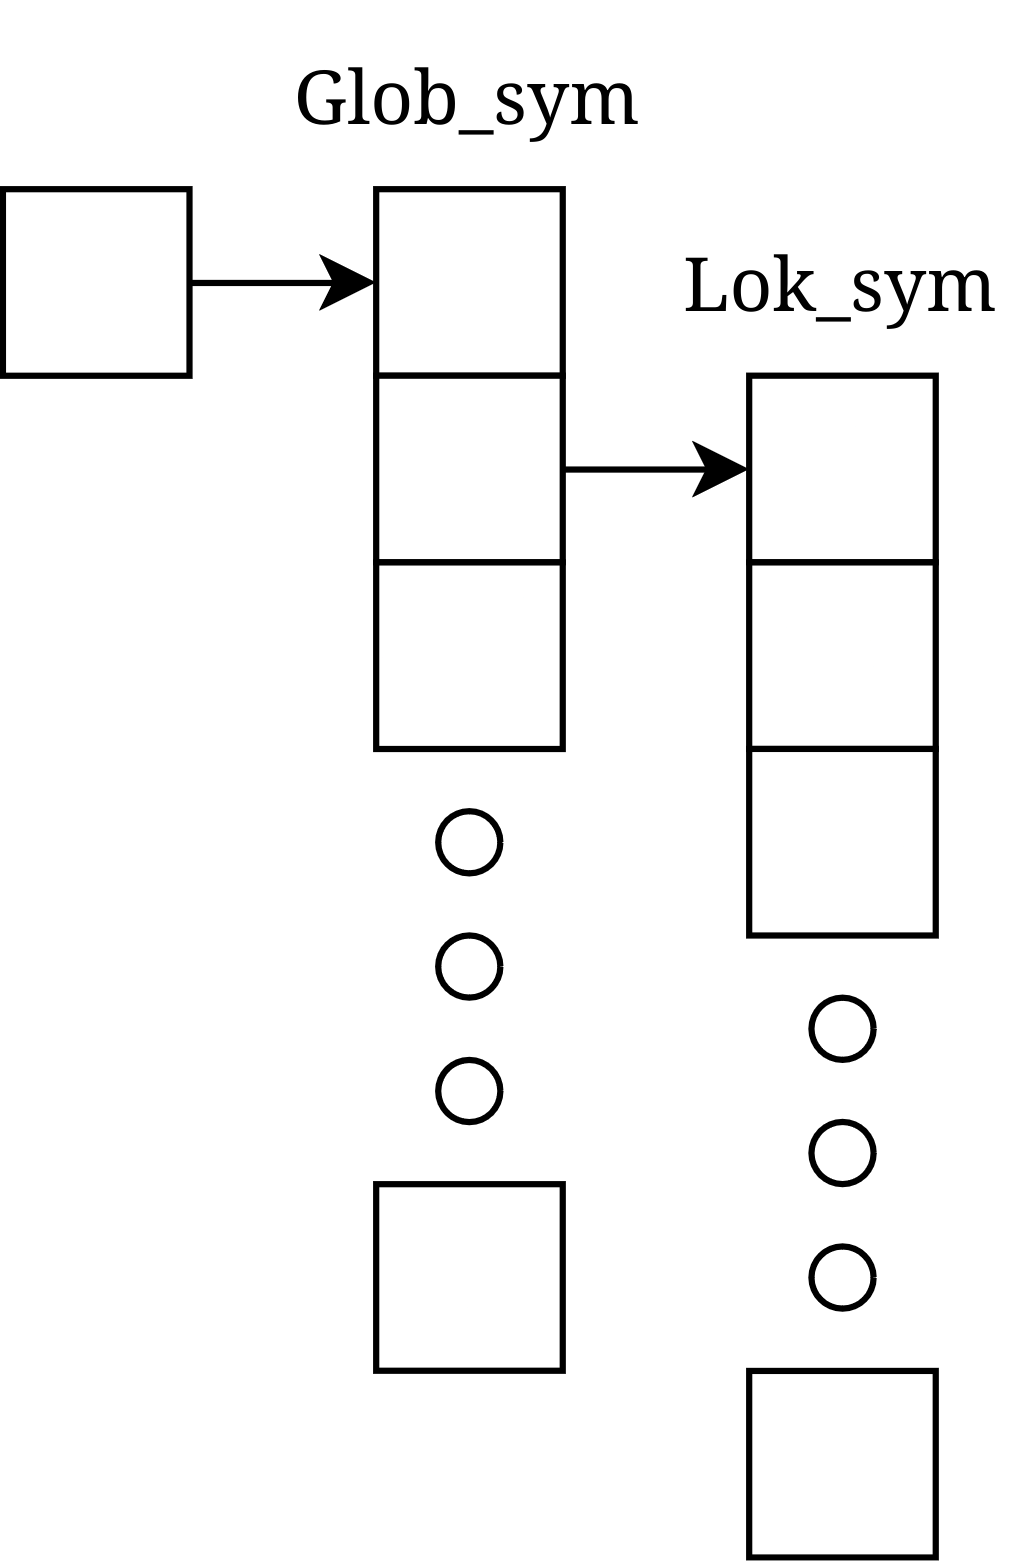
\includegraphics{diag.png}}
			\caption{Tabulka symbolov}
		\end{wrapfigure}
	Tabulku symbolov sme implementovali podla zadania ako hašovaciu tabulku. V prekladači existuje ukazaťeľ na \textit{globálnu tabulku} v ktorej sú záznami definovaných funkcií. Každá funkcia má v sebe odkaz na \textit{lokálnu tabulku} symbolov.  Lokálna tabulka symbolov, obsahuje záznami premenných v daných funkciách. Parametre funkcie sú na začiatku tiež interpretované ako lokálné premenné. Zauímavosťou je určite riešenie rozsahu platnosti lokálnych premenných.
	 Namiesto riešenia zásobníku tabuliek symbolov, sme vymysleli jednoduchý systém, kde každá premenná má svoj vlastný zásobník čísiel. Tento zásobník určuje 
	 rozsah premennej následovne: Premenné definované v tele hlavnej funkcie majú velkosť zásobníku 1 a na zásobníku je čislica 1, Pokiaľ definujeme premennú v neakom podbloku, tak na zásobník vložíme hodnotu ktorá je jedinečná pre daný podblok (ilustrujeme obrázkom). Tabulka je kvôli požadovanému implicitnému
	 zreťazeniu obmedzená na 1000 položiek, čo si uvedomujeme že nie je najvhodnejšie riešiene, avšak veríme že pre projekt bolo dostačujúce. 
	 \\
	\begin{figure}[ht]
		\begin{center}
			\scalebox{0.28}{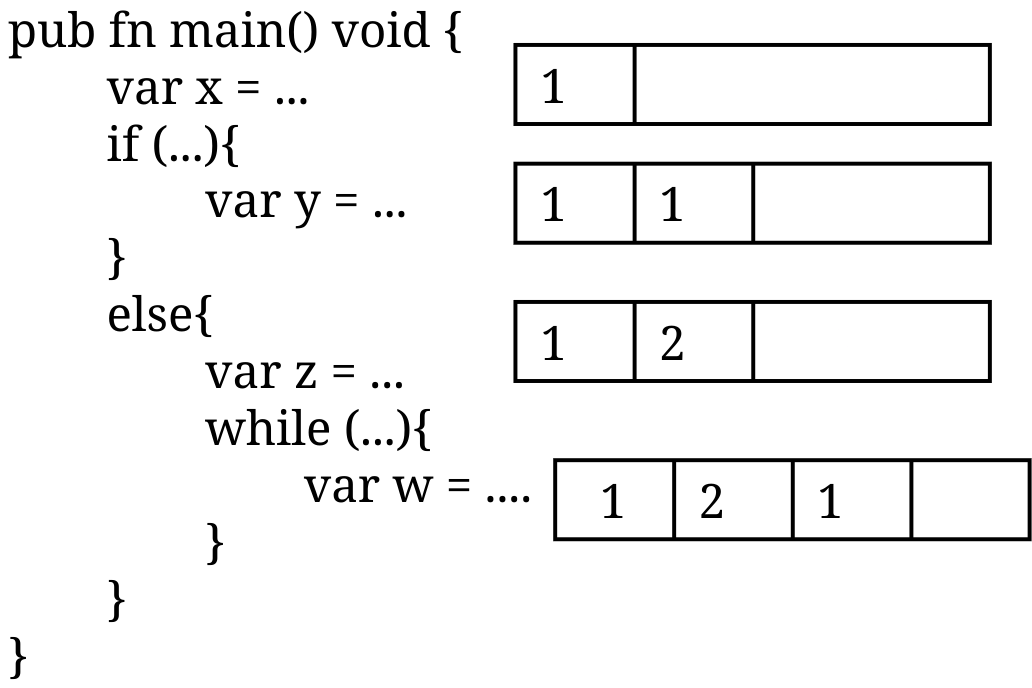
\includegraphics{sada.png}}
			\caption{Riešenie rozsahu platnosti}
		\end{center}
	\end{figure}
	\newpage

	\subsection{Implementácia ostatných častí}
	Ostatné časti (Skener, Parser, Generácia kódu, Zásobník, fronta) sú implementované štandardne metódami prednášanými na FIT VUT, preto ich špecifikáciu
	vynecháme.  
	
	\section{Práca v tíme}
	Na projekte sme pracovali počas celého semestra. Na správu verzií sme využívali platformu GitHub, ktorá nám umožnila prehľadnú organizáciu zdrojového kódu, sledovanie zmien a jednoduché riešenie prípadných konfliktov v kóde. Vďaka tomu mal každý člen tímu vždy prístup k aktuálnej verzii projektu. Na komunikáciu sme používali Discord, ktorý nám poskytol priestor na rýchlu výmenu informácií, plánovanie úloh a riešenie problémov v reálnom čase. Táto platforma bola užitočná najmä pri každodennom zdieľaní poznatkov alebo konzultáciách ohľadom implementácie jednotlivých častí projektu. Okrem online komunikácie sme sa raz týždenne stretávali osobne, aby sme spoločne zhodnotili doterajší pokrok, stanovili priority na nadchádzajúce obdobie a riešili zložitejšie časti projektu, ktoré si vyžadovali detailnú diskusiu. Tento pravidelný rytmus spolupráce zabezpečil plynulý vývoj projektu a pomohol nám efektívne rozdeliť prácu medzi jednotlivých členov tímu. Navyše sme sa rozdelili do tímov po dvoch podľa toho, ako sme ubytovaní na internátoch, čo nám umožnilo ešte rýchlejšiu komunikáciu pri problémoch špecifických pre jednotlivé tímy.
	
	\newpage
	\section{PRÍLOHA A - Konečný automat}
	
	\newpage
	\section{PRÍLOHA B - LL1 gramatika}
	
	\newpage
	\section{PRÍLOHA C - LL1 tabulka}
	
	\newpage
	\section{PRÍLOHA D - Precedenčná tabulka}
	
\end{document}